\section{实验步骤}

本章节将展示本系统的实验步骤,包括分布式架构的设计和实现,与数据库系统的设计和实现。

\subsection{分布式系统的设计}

\begin{figure}[H]
    \centering
    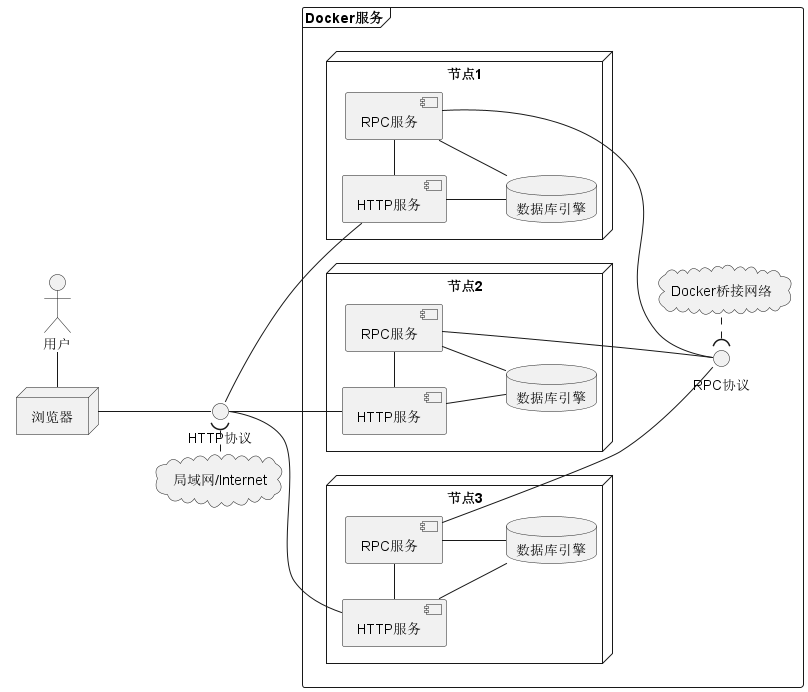
\includegraphics[width=\linewidth]{examples/分布式系统架构.png}
    \caption{分布式系统的架构}
    \label{fig:dist-arch}
\end{figure}

如图\ref{fig:dist-arch}所示,该系统的总体架构是B/S架构,用户可通过浏览器,基于HTTP协议,通过局域网或Internet与服务端进行交互,服务端对用户来说完全透明。

服务端内部则是分布式架构,不同节点拥有独立业务逻辑,能够完成完整的数据存储和读取业务。节点通过HTTP服务接收用户请求,之后与本地的数据库引擎(后续章节中会详细介绍)进行交互来完成数据的存取。

当节点数量不只有1个时,节点之间就可以通过RPC服务进行通信。当请求通过哈希函数分配给本机时,节点会自行处理逻辑,否则就会通过RPC发送给目标节点进行处理,并接收其返回值再返回到用户。节点之间通过Docker桥接网络进行通信。

本系统可分为3个模块:
\begin{itemize}
    \item HTTP服务(HTTPService)。该模块负责接收的HTTP请求,并选择处理请求节点。
    \item RPC服务(RPCService)。该模块负责接收并处理RPC请求。
    \item 数据库引擎(KVService)。该模块负责存取数据,在后续章节会详细介绍。
\end{itemize}

\subsection{分布式系统的实现}

分布式系统对外通过HTTP协议进行通信,从而接收用户命令以进行处理。

\begin{figure}[H]
    \centering
    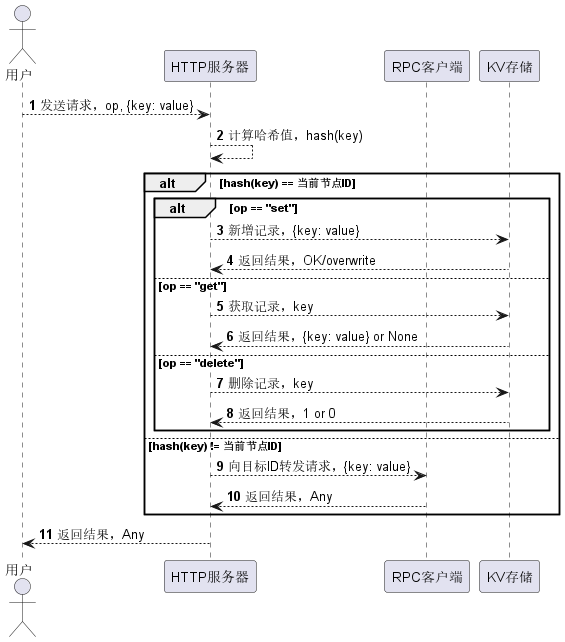
\includegraphics[width=0.8\linewidth]{examples/接收http流程.png}
    \caption{接收HTTP请求流程}
    \label{fig:recvhttp}
\end{figure}

图\ref{fig:recvhttp}描述了任一节点接收HTTP请求的详细流程。当用户向任意服务器节点发送HTTP请求后,该节点通过对键进行哈希函数获得唯一ID。如果ID与本地ID匹配,则与本地KV存储进行交互,通过操作字段op判断操作类型,之后选择对应的方法。如果ID与本地ID不匹配,则通过RPC客户端将请求转发给目标远程服务器。

分布式系统内部通过RPC协议进行通信,如果用户请求需要进行转发,就会通过RPC客户端向对应服务端的RPC端口发送请求,从而调用对应节点的函数来执行请求。

\begin{figure}[H]
    \centering
    \includegraphics[width=0.8\linewidth]{examples/接收RPC流程.png}
    \caption{接收RPC请求流程}
    \label{fig:recvrpc}
\end{figure}

图\ref{fig:recvrpc}描述了任一节点接收RPC请求的详细流程。当RPC服务端收到来自任一节点的RPC客户端发送的RPC请求后,服务端所在节点就会通过操作字段op判断操作类型,并于本地KV存储交互,之后把请求返回给RPC客户端。

下面是代码的展示。为了清晰明了的介绍代码逻辑,这里仅展示简化后的代码,完整代码请见附录。

\begin{lstlisting}
import uvicorn
from fastapi import Fastapi

app = Fastapi()

@app.post('/')
def handle_set(data: Dict):
    for k, v in data.items():
        return service.handle_http_req('set', k, v)

if __name__ == '__main__':
    uvicorn.run(app, port=<HTTP_PORT>)
\end{lstlisting}

上面的代码清晰展示了HTTP服务的建立流程。只需导入fastapi和uvicorn包,创建app,设定路由,最后通过uvicorn启动app即可。

\begin{lstlisting}
from rpyc import Service
from rpyc.utils.server import ThreadedServer

class RPCService(Service):
    def exposed_handle_rpc_req(self, op, k, v=None):
        func = getattr(self, 'do_' + operation)
        return func(k, v) if v is not None else func(k)

if __name__ == '__main__':
    service = RPCService() 
    rpc_server = ThreadedServer(service, <RPC_PORT>)
    t = threading.Thread(rpc_server.start, True)
    t.start()
\end{lstlisting}

上面的代码清晰展示了RPC服务的建立流程。Rpyc框架可以直接暴露继承自Service类下开头为exposed\_的方法,这样来自其他节点的客户端可以直接通过方法名使用该方法。该方法会通过op字段获取本地的set/get/delete等方法句柄,之后调用该方法获得结果。需要注意的是,RPC服务在一个额外线程上启用,这样才能与HTTP服务器同时运行。

\begin{lstlisting}
class Node(object):
    def handle_http_request(self, operation, k, v=None):
        target_id = self._select_rpc(k)
        if self._is_local(target_id):
            return self.handle_local_req(operation, k, v)
        else:
            target_host = self.hosts[target_id]
            conn = rpyc.connect(target_host, <RPC_PORT>)
            return conn.root.handle_rpc_req(operation, k, v)
        
    def _select_rpc(self, k):
        return hash(k) % len(self.hosts)

    def _is_local(self, id_):
        return id_ == self.id
\end{lstlisting}

上面的代码展示了节点的选择和转发策略。其逻辑非常简单,首先根据hash()函数获取唯一ID号,当ID与本地ID匹配时,就调用本地的处理函数;否则,向ID对应的目标节点转发RPC请求。

\subsection{数据库系统的设计}

\begin{figure}[H]
    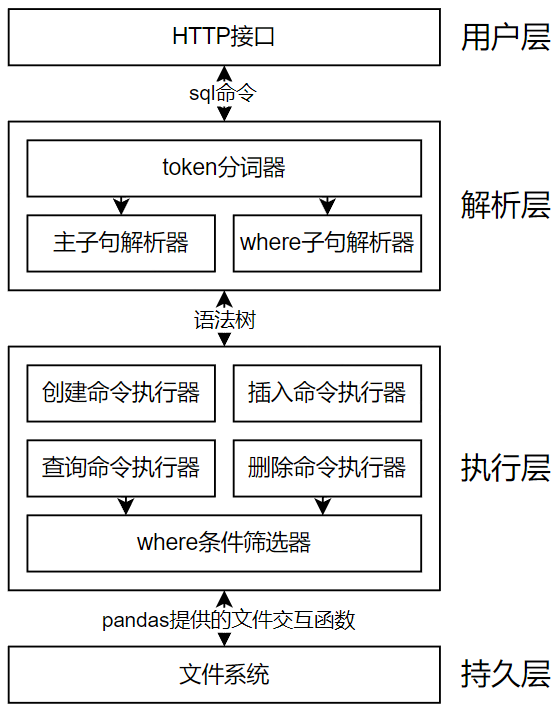
\includegraphics[width=0.5\textwidth]{examples/数据库系统架构.png}
    \centering
    \caption{数据库系统架构}
    \label{fig:db-arch}
\end{figure}

如图\ref{fig:db-arch}所示,由于数据库系统非常复杂,这里以分层架构实现。本系统中的数据库系统共4层,分别为用户层、解析层、执行层、持久层,各层功能如下:
\begin{itemize}
    \item 用户层。负责接收用户的HTTP请求,提取其中的sql命令并传递给解析层,之后将结果返回给用户。
    \item 解析层。负责解析sql命令,包括分词、主子句解析和where子句解析,由于where语句比较特殊,这里单独进行解析。解析后的sql命令以语法树的格式传递给执行层。
    \item 执行层。负责执行各种类型的sql命令,包括创建命令、插入命令、查询命令、删除命令,以及where条件的筛选策略。将语法树转换为与文件系统的若干交互函数。
    \item 持久层。负责存放表结构和内容在文件系统中。
\end{itemize}

\subsubsection{Sql命令的解析}

Sql命令的解析是本数据库系统的核心部分,这里详细介绍其解析算法。首先是分词逻辑:
\begin{enumerate}
    \item 对于"(",")",",",";"等特殊符号,在其两端添加空格。
    \item 对于">","<","=","<=",">="等特殊符号,去掉两端的空格(如果有)。
    \item 以空格作为分隔符,将命令字符串分割为若干token,并去掉长度为0的token,得到token序列。
\end{enumerate}

完成分词之后,需要向token序列中插入一些特殊的指示token,如fields/table等,具体的指示token和要插入的位置如表\ref{tab:token}所示。

\begin{table}[H]
    \centering
    \caption{指示token插入位置与偏移量}
    \label{tab:token}
    {
    \begin{tabular}{|c|c|c|}
        \hline
        指示token & 被插入的token & 插入偏移量 \\
        \hline
        fields & select & 1 \\
        fields & into & 2 \\
        fields & table & 2 \\
        table & into & 1 \\
        table & from & 1 \\
        $($ & table & 1 \\
        $($ & * & 0 \\
        $)$ & table & 3 \\
        $)$ & * & 1 \\
        \hline
    \end{tabular}
    }
\end{table}

其中指示token表示要插入的特殊token,被插入的token表示哪些token需要被插入特殊token,插入偏移量表示插入的特殊token相对于被插入token的位置。对于每个sql命令来说,上述指示token会由上至下逐个执行。

例如,对于命令select * from user;来说,select之后1格被插入fields,from之后1格被插入table,table之后1格被插入(,之后3格被插入),*之后0格被插入(,之后1格被插入)。于是原命令变为:select fields ( * ) from table ( user );

完成token处理之后,就要将其转化为语法树结构,这一步的逻辑是:
\begin{enumerate}
    \item 首先创建一个root节点,并记录根节点为当前父节点。
    \item 从左到右逐一遍历所有token,并记录当前token的上一个token:
    \begin{enumerate}
        \item 如果该token是"(",则将上一个token设为当前父节点。
        \item 如果该token是")",则将当前父节点的父节点设为当前父节点。
        \item 否则,将当前节点追加为当前父节点的子节点。
    \end{enumerate}  
\end{enumerate}

经过上述逻辑之后,select, fields, from, table被设为root的子节点,*被设为fields的子节点,user被设为table的子节点,即:

\begin{lstlisting}[language=bash]
root
|
+-- select
+-- fields 
|   +-- *
|
+-- from
+-- table
    +-- user
\end{lstlisting}

上述策略是普通语句的解析逻辑,然而对于where子句来说,其解析逻辑有所不同。对于where子句来说,逐步遍历其token,如果当前token为and/or/not等逻辑运算符时,就要寻找该运算符的上一个数学运算集合和下一个数学运算集合。具体来说:

\begin{itemize}
    \item 从逻辑运算符向前搜索,如果上一个符号为")",则需要找到匹配的"(",则括号包裹的集合即为上一个数学运算集合。如果上一个符号不为")",则上一个<field><op><value>(如id=1)形式的数学运算单元即为上一个数学运算集合(<op>表示>,<,=,>=,<=等运算符号)。
    \item 从逻辑运算符向后搜索,如果上一个符号为"(",则需要找到匹配的")",则括号包裹的集合即为上一个数学运算集合。如果上一个符号不为"(",则上一个<field><op><value>形式的数学运算单元即为上一个数学运算集合。
\end{itemize}

在找到上一个和下一个数学运算集合之后,需要执行替换顺序和添加特殊符号的操作,从<set1> <op> <set2>变为<op> (<set1>, <set2>),这样就完成单一逻辑运算符的变换。

以name="user" and (id=1 or id=2)为例,首先遍历到逻辑运算符and。其上一个集合为name="user",下一个集合为(id=1 or id=2)。于是变为

and ( name="user", (id=1 or id=2) )。

之后遍历到逻辑运算符or,并进行相同操作,最终得到

and ( name="user", or ( id=1, id=2 ) )。

最后,上述where子句可以通过同样的语法树生成逻辑得到语法树:

\begin{lstlisting}
root
|
+-- and
    +-- name="user"
    |
    +-- or
        +-- id=1
        +-- id=2
\end{lstlisting}

需要强调的是,语法树的生成策略和形式多样,这里的生成策略只是本系统原创的一种策略。

\subsubsection{Sql命令的执行}

Sql命令的执行相对简单,只需要挑选出语法树中所需要的字段,并进行相关操作即可。

例如,对于命令create table user (id, username, password),其语法树的形式如

\begin{lstlisting}
root
|
+-- create
+-- table 
|   +-- user
|
+-- fields
    +-- id
    +-- username
    +-- password
\end{lstlisting}

于是通过遍历root下面的各个节点,很容易可以得到操作类型为create,表名为user,字段名有id, username, password,之后就可以调用pandas相关函数创建一个数据帧,并调用导出函数保存到本地文件系统中。

需要特殊说明的是where子句的执行流程。对于拥有where条件的sql命令来说,本系统采用后过滤的策略。系统首先查询得到完整的数据帧,并维护一个空列表,之后对where子句的语法树作后向遍历得到一个运算序列:

\begin{itemize}
    \item 如果当前运算是一个数学运算,如>,<,=等,则从数据帧中筛选出符合条件的行索引,并以集合形式存入列表中。
    \item 如果当前运算是一个逻辑运算,如and,or,not等,则对当前列表中的所有集合进行求交集、并集、差集的操作。
\end{itemize}

最终,列表中的第一个集合即为过滤后的索引,通过索引就可以得到过滤后的表信息。之所以以索引形式进行运算和存储,是为了减少空间消耗和运算量。

\subsection{数据库系统的实现}

Sql解析器的代码逻辑如下所示,为了简洁明了,这里仅展示简化后的代码,完整代码请参见附录。

\begin{lstlisting}
class SqlParser(object):
    def parse(self, sql):
        sql = self._handle_space(sql)
        tokens = self._split_to_tokens(sql)
        tokens = self._handle_special_tokens(tokens)

        root = Node('root')
        parent = root
        cur_node = None
        for token in tokens:
            if token == '(':
                parent = cur_node
            elif token == ')':
                parent = parent.parent
            elif token == ',':
                pass
            else:
                cur_node = Node(token, parent)

        return root
\end{lstlisting}

可以看出,sql字符串依次通过处理空格,切分为token序列,处理特殊token(指示token),组织为语法树4步。这里树结构采用了python的anytree库,使用非常方便。

Sql语句的执行代码如下所示,简单起见,这里仅展示select语句的执行逻辑:

\begin{lstlisting}
class Database(object):
    def __init__(self):
        self.parser = SqlParser()

    def exec(self, command):
        root = self.parser.parse(command)
        root = self._optimize_command(root)
        result = self._run_command(root)
        return result
    
    def _run_command(self, root):
        op = root.children[0].name
        if op == 'insert':
            return self._do_insert(root)
        if op == 'select':
            return self._do_select(root)
        if op == 'delete':
            return self._do_delete(root)
        ...
        return f'operation {op} is not supported!'
    
    def _do_select(self, root):
        table_name = self._get_values(root, 'table')
        fields = self._get_values(root, 'fields')
        table_path, is_exist = self._get_table_path(table_name)

        if not is_exist:
            return f'[ERROR] Table {table_name} is not existed!'
        
        df = self._read_table(table_path)
        
        if fields == '*':
            fields = df.columns.tolist()
        
        try:
            df = self._filter_where(df, root)
            df = df[fields].reset_index(drop=True)
            out = str(df) + f'\n{len(df)} rows selected.'
            return out
        except BaseException as e:
            print(e)
            return '[ERROR] Select failed! Maybe some fields are not in table!'
\end{lstlisting}

可以看出,sql命令经过解析、优化、执行三个阶段,执行时会根据语法树中根节点的第一个值(即操作类型)分配操作函数。对于select函数而言,会从语法树中获取表名、字段名等信息,并进行表不存在和查询失败的异常处理,和方言"*"号的替换处理。对于查询到的完整数据帧,会根据where子句进行过滤,最后返回指定列的内容。